\section{Introduction}

For the past few decades, both the field of computing in America and
computer science in higher education have suffered from significant
underrepresentation of women and domestic students of color.  A
wide variety of projects have attempted to address this issue.
However, even after all of these efforts, a recent Taulbee survey
still suggests that only 17.9\% of bachelor's degrees in computer
science are awarded to students identified as female, 3.1\% to
students identified as Black or African-American, and 7.5\% to
students identified as Hispanic \cite{Taulbee2016}.  More work is
needed.

Many factors are at play in this problematic situation.  One that
is repeatedly identified is a ``pipeline problem'', with members
of these groups deciding early on that they do not belong in computer
science \cite{Gurer2002}.  As a result, the broader compute science
community has tried a variety of outreach activities
\cite{McGill2015,Decker2016}.

Over the past three years, our research team has explored the effect
of summer code camps on student interest and self efficacy.  Rather
than employing the more common approaches to computing the emphasize
playful aspects of computing (e.g., through robots, games, or
Minecraft) \cite{code-camp-survey-sigcse-2017}, we emphasized
meaningful uses of computing \cite{arts-coding,dssg-sigcse-2018},
focusing primarily on issues of computing for social good
\cite{Goldweber2013}.  We hypothesize that these more meaningful
approaches will help build students' self efficacy and interest,
particularly among students from groups traditionally underrepresented
in computing.

In this paper, we focus on a pair of camps offered in summer 2017
and 2018 in which middle-school students explore computational
techniques related to the emerging field of data science.  and used
their newly-developed skills to explore data sets relating to issues
of social good.

In section 2 of the paper, we describe the local context of the
camp, particularly the characteristics of our community and the
students who enrolled.  In section 3, we describe the design and
structure of the camp and provide additional detail about our
approaches data science and computing for social good.  In section
4, we provide a broader view of the curricula of the two camps and
our rationale for updates between the two years.  In section 5, we
review data from camper surveys.  Finally, in sections 6 and 7, we
further consider the implications of the data and our observations
from the camp.

\section{Local context}

Our institution is in a rural community (approximately 10,000
residents) in a relatively white state---91.4\% of the population was
identified as white in the latest census.  Our community has a large
population of working poor: While the poverty rate in our county
is over 30\%, the unemployment rate is under 3\%.  Surrounding
communities have similar populations.

In designing the camp, we strove to address the particular concerns
of our community.  While we wanted to address the underrepresentation
of girls and students of color, we also wanted to make sure that
the camp was accessible to students of lower socio-economic status.
Building these students' self-efficacy seems particulary important
as the opportunities presented by computing careers can make a huge
difference in their lives.  We used a variety of approaches to
support these students, including free tuition for students on free
or reduced lunch programs\footnote{Unfortunately, because many feel
a stigma in our schools, many students who would qualify for these
programs choose not to enroll.  The problem is most significant at
the high-school level, but it is clearly also in play at the
middle-school level.  To help address that stigma, we relied only
on families' self reports on the application form, and not on data
from the school district.}, providing meals and snacks for every
camper, subsidizing costs for all campers, and providing no-cost
options for early drop-off and late pick-up.

Because there are few educational enrichment activities available
to rural students, we drew students not only from our own community,
but also from neighboring communities.  Some came from as far as
sixty miles away, suggesting that there are far too few such
opportunities for students in rural areas.

Thirty-eight campers signed up for the 2017 iteration of the camp, 
far more than we expected---many campers arrived on the first day
with a friend or relative who had heard about it from them and
wanted to sign up.  We had also received a number of prior requests
of the form ``I know I missed the sign-up deadline, but ...'', and
so knew that we would need to be prepared for this additional
interest.  Surprisingly, a smaller number signed up for the 2018
iteration.  That may have been due to a late announcement by the
local school districts.

In the first year of the camp, had a relatively diverse group of
campers for our area, with 82\% of campers identifying as white.
We had 37\% female campers which, while fewer than we had hoped
for, represents a relatively high number for what might seem a
technical subject.

\textit{TODO: Need to insert data for the second camp.}

Both college students and local high-school students served as
counselors for the camps.  We generally tried to maintain a ratio
of about one counselor per four campers in the classroom; that ratio
varied slightly as counselors took breaks or worked on preparation
for other activities.  As a result of this relativley low ratio,
counselors were able to provide support promptly and effectively.
And, because counselors were not pressed for time, they were able
to encourage campers to find answers to their problems themselves,
rather than provide immediate solutions.

\section{Designing the camp}

We had selected the high-level approach to the camp prior to the
research project.  Given the evidence of the value of computing for
social good approaches,\cite{Goldweber2013}, our team's experience
with such activities in a prior project,\cite{arts-coding}, and the
paucity of code camps that focus on computing for social
good,\cite{code-camp-survey-sigcse-2017}, we chose to include
computing for social good as a core theme of the camp.  At the same
time, we wanted to expose students to some current approaches to
computing.  Since our institution has begun a new data science
initiative, it seemed appropriate to make data science the second
core focus of the camp.  The combination places our camp in a growing
``data science for social good'' (ds4sg) movement.\footnote{E.g.,
\texttt{https://dssg.uchicago.edu/data-science-for-social-good-conference-2017/}.}

But a camp is more than its themes.  We also identified learning
outcomes, design a curriculum, and develop projects.  In the remainder
of this section, we explore the two themes and these additional
issues in more depth to inform those who might wish to design their
own camps.

\subsection{Themes}

\subsubsection{Computing for social good}

As Goldweber \textit{et al.} \cite{Goldweber2013} suggest, many women
and students of color often avoid computing because they perceive
that computing is incapable of making a difference in their primary
areas of interest.  That is, unlike many of the students who
traditionally study computer science Such students often seek out
careers which have the potential of positively impacting their
communities.  Hence, unlike students who enter computing because
of a background in tinkering with computers or computational tasks,
these students need to see that computing can have a positive impact
on the world.  To encourage a more diverse discipline, we developed
the camp around Goldweber's premise of ``computing for social good''
(CSG) \cite{Goldweber2015}, in which problems and context suggest ways
in which computing can have a real impact on the world.  This
approach promoted the social relevance of computer science while
maintaining foundational programming concepts to give campers a
broader and more informed perception of computer science as a whole.

The direct application of the CSG methodology to the camp provided
much of its content. For example, Goldweber's ``Reuniting Families''
learning helped us teach campers about developing algorithms in the
context of societal disasters; we added a kinisthetic component to
that activity so that students not only designed algorithms for
reuniting families, but also carried out each others' algorithms
in a large public space.  Our discussions about the current and
future roles of technology encouraged campers to explore computing
solutions to personal and societal issues.  Similarly, case studies
about weather patterns and car crashes favored an analytical approach
to national events.

\subsubsection{Data science}

Although the field of data science is rapidly gaining in popularity,
its definition is tenuous, at best.  As one of the statistics faculty
noted when talking to us about possible ways to design a data science
curriculum, ``if you ask a dozen statisticians to define data
science, you'll get at least a half-dozen different answers''.
Particularly since we were focusing on the computational aspects
of data science, we chose two primary ways of thinking about it:
We taught students that data science is a field in which you gain
insight from existing data and that data science requires a series
of replicable processes (e.g., cleaning and wrangling) carried out
by algorithms that data scientists design and implement.  We focused
on how the components of algorithms (e.g., conditionals,  loops,
and subroutines) can be used to navigate and a data set and how,
along with visualization routines, help one develop a broader understanding
of data and share that understanding with others.

Although our institution's new data science initiative provided one
motivating factor for teaching data science, it was not the only
reason.  Our choice to emphasize the topic in this camp stemmed
from its ability to further expand campers' perceptions of the
capacity of computer science and computing to help people solve problems
and to make a difference.

The theme of data science compelled us to design the camp around
data analysis and exploration. As a result of this, we spent much
of the week teaching campers practical data organization and
manipulation skills that would allow them to delve into datasets
on their own.

\subsubsection{Combining the themes: Data science for social good}

At the time we were designing the first offering of the camp, we looked
for a short and pithy title that covered the two core aspects of the camp.
We settled on ``Data science for social good''.  At the time, the
new field with the same name was just beginning.  As in the cases of
both data science and computing for social good, it appears that there
are a wide variety of meanings associated with these terms.

\textit{TODO: Find some of the primary initiatives and grab 
text from there.}

In choosing our own approach to computing for social good, we
identified a variety of approaches to help students understand how
the tools of data science can have an impact.  For example, although 
much of our focus was on students writing scripts to explore and
visualize data, we also exposed them to mechanisms for gathering
environmental and other data.  The latter approach helped them understand
that they need not rely only on extant data sets, but could also
create their own.  In fact, two sets students designed their own attitudinal
surveys as part of their broader projects.

More generally, it appears students came to understand that the
tools they were learning allowed them to identify or gathering data
relevant to a social or societal situation of interest and transform
those data into a form in which one could make arguments relevant
to that situation and to change opinions.  Focusing on computing
for social good also helped us avoid some of the stigma that may
be associated with data science, the sense that data science most
frequently means ``companies like Amazon and Facebook using their
data to sell you something''.  Like all projects in computing for
social good, our focus on ds4sg provided students with the opportunity
to think about issues that mattered to them.

\subsection{Platforms and languages}

We took particular care in selecting applicable programming languages
and intuitive platforms. Other concerns regarding this choice
included disparities in campers' prior programming experience and
their broad age range. For reasons which will be introduced and
elaborated in the following sections, we chose to base our camp in
two main languages: A pair of block-based languages and Python.

\subsubsection{BBC micro:bits---Hands on activities with a block-based language}

BBC micro:bits are cheap, pocket-sized programmable computers
designed to act as an introductory interface for novice programmers.
Each individual micro:bit has a five-by-five grid of LEDs forming
a graphic interface, with two programmable buttons on either side
for user input.  The small size of the micro:bit might be deceiving
due to its numerous additional features including a built-in radio,
compass, and Bluetooth.\footnote{http://microbit.org/about/}

We introduced the micro:bit Blocks Editor early on in the week in
to provide an intuitive environment to introduce key programming
concepts such as loops, conditionals, and variables.\footnote{For
reasons that we do not quite understand, the block language does
not currently support subroutines.} While the block-based language
supported the novices among our students, since some students had
used a block-based language in the past, the use of a new block-based
language also served as a review in writing algorithms for campers
who had prior experience with programming, while the novice coders
in the camp were able to catch up. The micro:bits served as a visual
counterpart to indicate their progress, both successes and failures.
As one of our primary goals of the camp was to increase the campers'
confidence in the subject matter, it was important to give the
campers a sense of accomplishment in a tangible and results-oriented
way early on.

\subsubsection{Jupyter Notebook---Programming like a data scientist}

As we had hoped, the Data Science for Social Good Camp drew in
students who had not written much code before.  However, it also
appealed to students who had learned block programming languages
in schools and wanted to move up to a higher-level language.  At
the same time, we wanted to empower both sets of students to think
of themselves as real programmers.  For these reasons, we looked
to a platform that would permit students to write realistic data
science code but without too much overhead.  Because Python has
long-standing success as a text-based introductory language
\cite{Guo2014}, we settled on Python.  To provide students with the
opportunity to continue their work after the camp, we looked for a
cloud-based platform.  Many students do not necessarily have access
to their own computers.  Those that receive computers from the local
school district do not have the ability to install their own software.

Because of these issues, we selected the Jupyter
Notebook\footnote{https://jupyter.org/documentation.html} environment
for the students.
Jupyter Notebook is a Web-based platform for exploring and analyzing
data.  Like many modern computational systems for exploring data, it
allows the user to mix code, output, formatted text, and more into
something much like a scientist's notebook, but an interactive one.
Jupyter is a popular program among many professional data scientists.

Camp worksheets were comprised of a single Jupyter Notebook filled
with instructions, resources, and fill-in-the-blank partial code.
These worksheets supplied campers with the means to practice concepts
relating to data science, including a final analysis of their data.
Four out of the five days of camp, campers downloaded data from a
.csv or Excel document, computed summary statistics, and created
visualizations as prompted by counselor-made worksheets. The partial
code provided examples of syntax and common practice for code
organization, that served as a reference for campers in later, more
challenging exercises.

\subsubsection{Bridging the gap---From blocks to text}

To help campers adapt to a new programming environment, we designed
the camp to help them bridge the gap between the JavaScript Block
Editor for micro:bits and Jupyter Notebooks which focused less on
syntactic differences and more on the consistency of algorithmic
reasoning.  We scheduled the transition early in the week so that
campers would have more time to become comfortable with Python
before beginning their final projects.

We first used the BlockPy\footnote{https://think.cs.vt.edu/blockpy/index/}
Web-based Python Block Editor to familiarize campers with Python
\cite{Bart2017}.  BlockPy maintains the key infrastructure that we
had covered with campers in the micro:bits, such as loops, variables,
and conditionals, while introducing a split screen that displays
Python code alongside the block programs. In introducing BlockPy,
we had campers explore and compare the new interface to the old as
they looked for pieces of code that would help them solve a multi-part
word problem. This search allowed campers to reaffirm foundational
computer science concepts and develop their deductive skills.

Secondly, we implemented a review of BBC micro:bits in the middle
of the week using the micro:bits Python Editor. During this activity,
the campers were given documentation and example code so that they
could code their micro:bits into compasses, radio communication
devices, and more. Reexamining the capabilities of micro:bits gave
campers an intermission from new material as well as the opportunity
to get more hands on experience with Python.

\subsection{Final projects}

Early on in designing curricula, we decided to end the week with a
larger, more personally driven final project, which we titled ``Final
Findings'' and introduced on the first day of camp.  This project
was intended to leave the campers with a tangible example of the
skills they had acquired over the course of the camp and a way to
make a connection to the material.

To enhance their feelings of accomplishment, we concluded the camp
with project presentations in which pair of campers presented the
data they chose to analyze, the significant data they discovered
through calculations, and the visualizations that they programmed.
After their hours of work on the data, campers readied their materials
for presentation to others.  We invited parents and community members
to those presentations, which were a highlight of the week, which
gave our students an audience of roughly 80 people.  We discuss the
projects and presentations further in section 5.

\subsection{Structuring topics and days}

In designing the camp, we considered both technical outcomes---core
computational techniques like conditionals, loops, and subroutines--as
well as more conceptual outcomes---we wanted students to feel the
power that comes with writing programs and to realize that they had
the ability to write such programs.  We had also identified a
necessary set of skills for students to complete the final projects
in data science.  As is the norm in designing such camps, we then
considered the natural flow of ideas, reflecting on the transition
from block-based languages to a text-based language and an appropriate
spiral approach that helped students revisit topics in different
levels of depth.

While our primary focus was on computing topics, we knew from past
experience in this camp and others that students of this age group
would not learn well if they spent the day in front of the computer.
Hence, the camp schedule incorporated frequent ``away from computer''
activities including short breaks to play active and engaging games.
Snacks were offered during one of the breaks before lunch, and
another after lunch.

Moving the activities away from the computer did not mean that we
necessarily moved them away from thinking about core topics.  For
example, one the first day of camp we moved to an outdoor amphitheater
to carry out the algorithms they had developed for reuniting families
after a disaster.  We also included CS Unplugged \cite{csunplugged}
activities to introduce Computer Science concepts in a fun and
active environment.  During afternoon breaks, we invited faculty
and students in the Computer Science department to introduce campers
to their research.  

We also exposed students to the broader view of ds4sg early and
repeatedly.  Most days, counselors presented a case study that
integrated new concepts with social good data. For example, our
second case study taught campers how to organize data about weather
changes in a way that would allow them to analyze it in Python.
Most of the last day was devoted to working on final projects,
getting them ready to present to their friends and family.

\section{Camp structure}

\section{Assessment}

In order to measure the campers' change in self-efficacy and coding
confidence in a quantitative manner, we used pre- and post-survey
instruments based on upon the Georgia Computes! instruments
\cite{Bruckman2009} that ask students to respond to various statements,
such as ``I look like a computer scientist'' and ``I like the
challenge of computing'' on a seven-point Likert scale.  The questions
appear in fig.~1.  Through these surveys, we were able to get a
good sense of what subjects and concepts the campers were comfortable
with prior to attending the camp, so as to measure any significant
changes in their outlook by the end of the camp.  

\begin{figure}
{\small
1:\textit{I look like a computer scientist.} \\
2:\textit{Boys can do computing.} \\
3:\textit{Girls can do computing.} \\
4:\textit{I know a lot about computing.} \\
5:\textit{I can become good at computing.} \\
6:\textit{I know more than my friends about computers.} \\
7:\textit{I like the challenge of computing.} \\
8:\textit{Computer science is cool.} \\
9:\textit{I feel comfortable using a computer.} \\
10:\textit{I want to have a job in computing.} \\
11:\textit{I want to learn more about computing.} \\
12:\textit{Computer scientists are creative.} \\
13:\textit{Solving problems is fun.} \\
14:\textit{Computing is collaborative.} \\
15:\textit{I like computing.} 
}
\caption{Survey statements}
\end{figure}

\begin{figure}
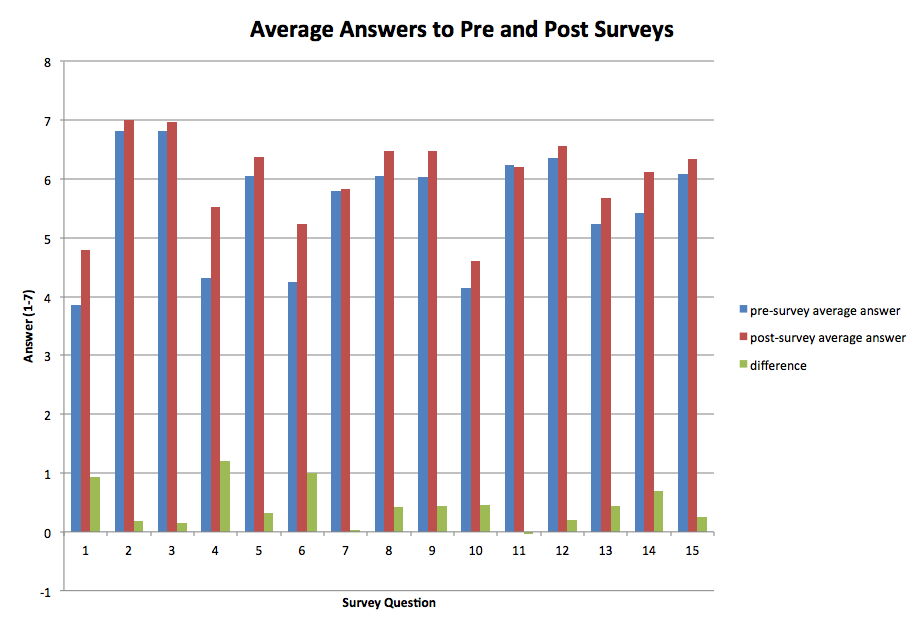
\includegraphics[width=3.3in]{images/AvgAnswersAll}
\caption{Student responses on pre- and post-surveys}
\end{figure}

In 14 out of the 15 questions, we saw an increase in the
average response (fig. 2), 8 of those changes were statistically
significant ($p < 0.05$). Notable positive changes (with t-test
results far below the threshold of significance) occurred in the
following questions: 1:\textit{I look like a computer scientist}, which
had a positive difference in average survey response of approximately
.94 points, 4:\textit{I know a lot about computing}, which had a positive
difference of approximately 1.2 points, and 6:\textit{I know more than
my friends about computers}, with a positive difference of 1 point.
It seems that campers, although somewhat apprehensive of their own
potential at the start of the project, found themselves more sure
of their abilities, not only in comparison with their peers outside
of the project, but also as independent thinkers.

Our surveys also included fields for ethnicity and gender, which
we hoped to use to investigate the differences of growth in
self-efficacy within different identity groups in early computer
science exposure. Due to the low representation of students of
color, we were unable to draw informative statistics on the growth
of the minority ethnic-identity groups within our project. We were,
however, able to investigate the differences in the growth of female
and male campers.

\begin{figure}
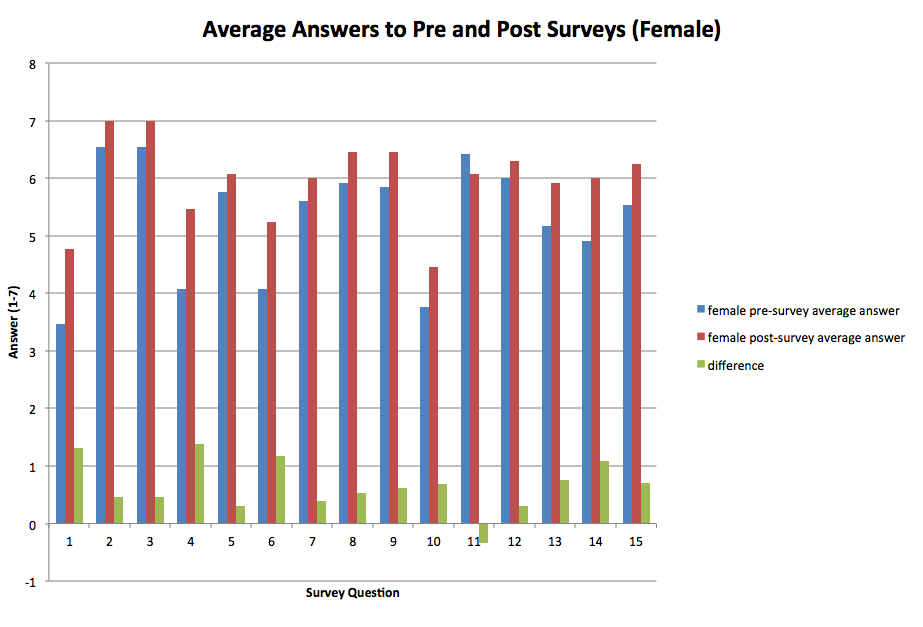
\includegraphics[width=3.3in]{images/AvgAnswersFemale}
\caption{Female student responses on pre- and post-surveys}
\end{figure}

\begin{figure}
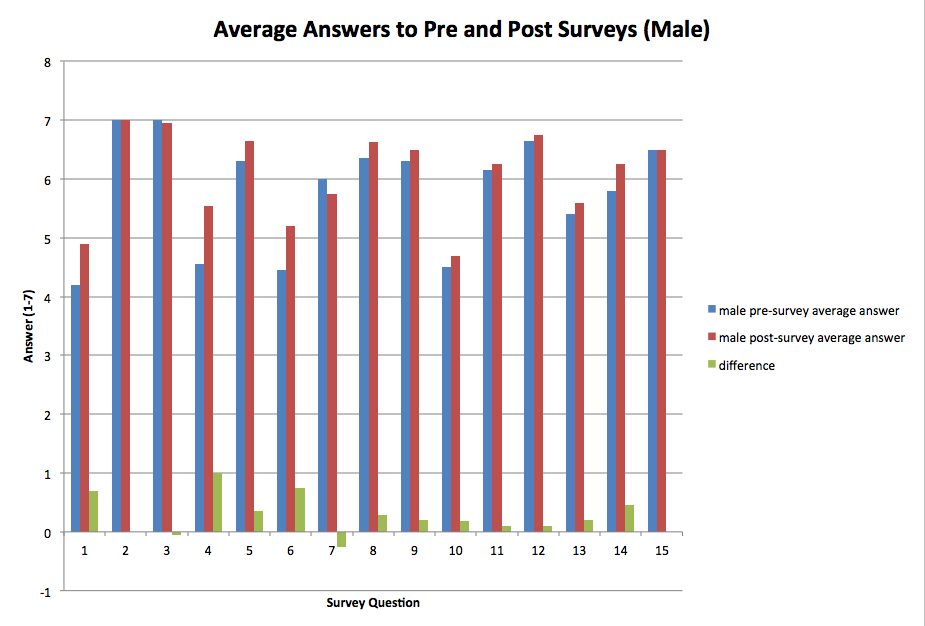
\includegraphics[width=3.3in]{images/AvgAnswersMale}
\caption{Male student responses on pre- and post-surveys}
\end{figure}

A few trends appeared when looking at the pre-survey and post-survey
averages for female campers (fig. 3) versus the averages for male
campers (fig. 4). Visually, it seems that although the female
campers averaged lower answers for most questions in both pre and
post surveys, they tended to have a larger increase in self-efficacy
than the male campers. This intuition is supported in the case of
questions 2:\textit{Boys can do computing}, 3:\textit{Girls can do
computing}, 7:\textit{I like the challenge of computing}, 9:\textit{I
feel comfortable using a computer}, 10:\textit{I want to have a job
in computing}, and 14:\textit{Computing is collaborative}, where
the change in the female campers' responses yielded significant
results ($p < 0.05$) and the change in male campers' responses did
not ($p > 0.05$). Only in question 5 did the male campers' difference
in average response yield a significant change while the female
campers' responses did not.

It seems that the curricula of this project had a more significant
effect on our female campers, which is in keeping with Goldweber
\textit{et al.}'s analysis \cite{Goldweber2013}.  The only negative
difference in averages in the female campers' responses occurred
with 11:\textit{I want to learn more about computing}, which,
although discouraging to note, did not yield significant results
when running a two-tail t-test (null hypothesis, $p < 0.01$).

Ultimately, we achieved our goal in increasing the self-efficacy
of the campers, and fulfilled our intent to make the concepts of
computer science more accessible to youth who perhaps do not identify
with the statement ``I look like a computer scientist''. The even
more significant increase in confidence in our female campers is
an especially encouraging outcome. Our results give us hope that
the campers left inspired, and may collaborate with peers outside
of the project to continue their education in computer science.

\section{Discussion}

As the assessment suggests, the camp was generally successful in
making a positive difference in students' sense of who can ``do''
computing and in their own self efficacy and interest.  While we
were saddened to see that the female students began the camp with
lower responses on most questions, we were encouraged to see their
gains as higher than the male student's.

However, many of our discoveries fell outside of the formal study.
One of the most telling came in the transition from micro:bits and
block-based programming to Jupyter and text-based programming.  We
had assumed that students would be excited by the micro:bits, and
they were, enough so that many parents contacted us to find out how
to get their own.  However, the students, by-and-large, told us
that they were more excited by the work they did in Python and
Jupyter Notebook.  Although we can not pinpoint the precise reason,
it seems that they felt like they were doing ``real'' programming
when they were working in Jupyter because the environment they used
matched that which working data scientists use.

We also encountered some significant challenges.  Different levels
of knowledge based on age group (rising 6th through 9th graders)
made it difficult to pace the introduction of new ideas and challenges
in such a way that it worked uniformly well.  In particular, the
rapid transition from block code to Python created syntactic
confusion.

The projects were central to the project and they provided some of
our greatest gains as well as our greatest stressors.
As campers gained familiarity with data science tools, they became
more comfortable with the idea of a final project on a subject of
their choosing. Rather than relying on a fixed collection of data
sets, we permitted campers to choose project ideas and then to
search for them.  When we held brainstorming sessions for project
topics, many campers demonstrated excitement and creativity in
choosing topics. Suggestions varied wildly; campers proposed to
study topics including the losses of monarch butterfly habitats and
migratory pathways, factors that contribute to video game sales,
implications of deforestation across the globe, and the associated
health risks of air pollution.  We were pleased to see that, even
at this age, students have social and societal topics that they are
passionate about.  Admittedly, there were a few groups who wanted
to work on more personal interests (video games, literature),
however, the vast majority clearly cared about societal topics and
found it valuable to be able to use computing to better understand
those topics.

However, we were also reminded of why many data science classes
provide students with a limited menu of data sets: most groups of
campers had difficulty locating datasets with appropriate and useful
data, even armed with the searching and vetting tools we taught
them.  Most groups found this experience quite frustrating.  Thus,
we counselors spent extra time finding datasets for some groups of
campers as they had been unable to find suitable data themselves.
This meant also that some groups had to change their topics depending
on the availability of the data that they intended to find.  For
example, a group interested in studying space debris ended up working
with a data set on UFO sightings.  Luckily, campers were gracious
and willing to adapt to these changes and most tackled their new
topics with vigor.

We were also quite pleased by the variety of ways in which students
approached the presentations, presentations which were clearly
intimidating to some.  Most used the features of Jupyter Notebook
to develop presentations that mixed code, graphs, and text.  Others
hand-drew posters.  And a few gave only oral presentations.  During
these presentations, the campers demonstrated knowledge and commitment
to their topics, in addition to budding presentation skills. While
there were some technical difficulties, such as a Jupyter notebook
that would not load, the campers performed well and took setbacks
in stride.

\section{Conclusions}

Although many middle-school outreach activities focus on students'
perceived interests, such as video games or ``exciting'' technologies,
it is clear from our experiences that computing for social good
provides a platform for helping students grow in self-efficacy and
interest.  We hope that our modest project will inspire others to
take a similar approach.

We have also found that while students can be intimidated by a text-based
programming language and a professional programming environment, they also
feel empowered and gain additional self efficacy in using such an environment.
While we are less comfortable recommending that others regularly take similar
approaches, our informal conversations with the campers suggest that the
approach is worth investigating further
